
\documentclass[man, 12pt, a4paper]{apa7}
\usepackage{geometry}
 \geometry{
 a4paper,
 marginparwidth=30mm,
 right=40mm,
 }

\usepackage[american]{babel}
\usepackage[utf8]{inputenc}
\usepackage{csquotes}
\usepackage{hyperref}
\usepackage[style=apa,sortcites=true,sorting=nyt, backend=biber, natbib=true, uniquename=false, uniquelist=false, useprefix=true]{biblatex}
\usepackage{authblk}
\usepackage{amsmath}
\usepackage{graphicx}
\usepackage{setspace,caption}
\usepackage{subcaption}
\usepackage{enumitem}
\usepackage{lipsum}
\usepackage{xcolor}

% Select what to do with todonotes: 
% \usepackage[disable]{todonotes} % notes not showed
\usepackage[draft]{todonotes}   % notes showed

% Select what to do with command \comment:  
% \newcommand{\comment}[1]{}  %comment not showed
\newcommand{\comment}[1]
{\par {\bfseries \color{blue} #1 \par}} %comment showed

\hypersetup{
pdfpagemode={UseOutlines},
bookmarksopen=true,
bookmarksopenlevel=0,
hypertexnames=false,
colorlinks   = true, %Colours links instead of ugly boxes
urlcolor     = blue, %Colour for external hyperlinks
linkcolor    = blue, %Colour of internal links
citecolor   = cyan, %Colour of citations
pdfstartview={FitV},
unicode,
breaklinks=true,
}

\DeclareLanguageMapping{american}{american-apa}
\addbibresource{references.bib}

\title{Social Integration of Migrants: A Systematic Review and Conceptual Framework}
\shorttitle{What is Integration?}

\author[1]{Jannis Kreienkamp}
\author[1]{Kai Epstude}
\author[1,2]{Laura F. Bringmann}
\author[1,2]{Peter de Jonge}
\affiliation{\hfill}
\affil[1]{University of Groningen, Department of Psychology}
\affil[2]{Some other affiliation}

\authornote{
   \addORCIDlink{Jannis Kreienkamp}{0000-0002-1831-5604}

  Correspondence concerning this article should be addressed to Jannis Kreienkamp, Department of Psychology, University of Groningen, Grote Kruisstraat 2/1, 9712 TS Groningen (The Netherlands).  E-mail: j.kreienkamp@rug.nl}

\leftheader{Kreienkamp}

\abstract{Abstract goes here.}

\keywords{Keyword \#1, Keyword \#2, ...}


\begin{document}
\maketitle

\todo[inline]{*Relevance*} 
The adaptation of migrants in new cultural contexts is an important issue in many societies around the world. With many of the migration push and pull factors in the economic, safety, social, and environmental domains becoming more severe, the topic is likely to become even more important in the future (Reference).
% Possible examples: violence and abuse of power (e.g., war, persecution; asylum seekers and refugees), social and economic disparities increasing (e.g., education, services, career; migrant workers, labor migrants), disproportionate environmental injustice (e.g., natural disasters, pollution, crop failure; environmental migrants). Together with population growth and globalisation.

With the current challenges and increasing migration it becomes even more important to understand how adaptation process unfolds and which aspects are most important to positive and sustainable outcomes.

\todo[inline]{*Problem*} 
One of the fundamental challenges to integration, faced by both researchers, practitioners, and policy makers, is an essentially scattered field with immense heterogeneity in definitions and measures of integration.
% Possible example: Definitions and measurements of integration have, for example, included aspects such as employment (Reference), housing (Reference), education (Reference), political participation (Reference), crime rates (Reference), language acquisition (Reference), values (Reference), well-being (Reference), stress (Reference), discrimination (Reference), social contacts (Reference), friendships (Reference), feelings of frustration (Reference), isolation (Reference), social functioning (Reference), and intergroup attitudes (Reference), the satisfaction belongingness needs (Reference), NEEDS (Reference).

The problem is not necessarily the diversity of important aspects but a missing framework to decide when certain measures are relevant and make sense of the large variation.

The aim of this paper is to offer a conceptual framework to analyse, measure, and understand the concept of individual cultural adaptation. Such a framework should be grounded in both psychological literature and the lived realities of a wide range of migrants.
\todo[inline]{*Proposal*} 
Migration is a complex transition experience that affects most areas of personal and social life. From such a person-centered perspective, we propose to use (1) basic dimensions of human experience and (2) domains of psycho-social functioning to build a bottom-up and inclusive framework of individual cultural adaptation.

\textbf{Dimensions:} We propose to use the basic elements of human experience and motivation to structure our understanding of the migration process. Many psychological models, across sub-fields, suggest that human experiences can be understood as consisting of affect, behavior, cognition, and desire components. Although the relative importance of any one dimension and the relationship between the dimensions may vary between contexts, the structuring properties of these four fundamental aspects is unaffected by context and relevant to any experience. As such, we can judge which part of the human experience is considered in the conceptualisation and measurement of cultural adaptation. Are we interested in behavioral adaptation (such as language use, or voting), in cognitive adaptation (such as identification with cultural values), in affective adaptation (such as feeling at home, or loneliness), in motivational adaptation (such as the satisfaction of competence or independence needs), or maybe a complex combination of any or all of these aspects?

\textbf{Domains:} Acculturation happens in different life domains \citep{Arends-Toth2006, Arends-Toth2007, Zane2004}. Different research teams have long advocated to conceptualise, investigate, and address separately within these domains of psychosocial functioning. As an example, \citet{Arends-Toth2006, Arends-Toth2007} suggest 15 public and private life domains (e.g., education [public], child-rearing [private]).

A person-centered framework based on core facets of the migrants’ social psychology and the environmental contexts of life domains would allow for a structured approach to evaluate existing definitions, measures, and interventions, but also offers a conceptual lens for building more comprehensive research and interventions.

This framework is not meant as an exhaustive or exclusive list of integration aspects but rather offers a structural framework to analyze and understand the broad experience of integration. Note that while any cultural adaptation process likely includes an emotional, cognitive, behavioral, and motivational change, the framework does not restrict which aspect of life caused the change. The relevant life domains will likely be different for different questions. As such, the framework does not speak to the multiplicity of specific physical, social, cultural, or spiritual challenges, but any such challenge should evoke negative response in affect, behavior, cognition, or desire.

Importantly this framework explicitly focused on the migrant's experience as the structuring experience. This is not meant to put the sole responsibility of "migration success“ on the newcomer or ignore the interconnectedness of intercultural exchange. We focus on the migrant experience as the structuring element because migrants usually find themselves in underprivileged positions. We also want to highlight that aspect of cultural adaptation that includes interconnected, co-dependent, or depend on the host majority members likely influence the individual experience of such situations (also across life domains).

why not meta analysis (too diverse and scattered)

\todo[inline]{*Structure of the manuscript*} 
\begin{enumerate}
  \item Past Literature on conceptualization and measurement (?)
  \item Focus group discussion
  \todo{Remove qualitative?} 
  \item Systematic review
   \begin{enumerate}
     \item methodological literature
     \item empirical literature
   \end{enumerate}
 \end{enumerate}

\section{Focus Group Discussion}
In a first step we reached out to societal stakeholder of the cultural adaptation process to gather information on key adaptation aspects in the lived realities out in the field.

We use these experience reports to explore the applied validity of our proposed framework. We expect … .
\subsection{Methodological Details}
participants

type of discussion

setup, consent, duration, …

coding- and analysis strategy

\subsection{Behavior}
most visible and often strong expectations

focus on social contact (direct and indirect functions)

language learning

domains important (school, work, sports, music, associations)

\subsection{Cognition}
how we think about ourselves and the world.

knowledge (navigational, social, cultural, lingual, norms)

identity (break in id, singular ‘refugee' id)

\subsection{Affect}
highlights importance of subjective experience

feeling at home and feeling accepted (often conditional on others)

feeling useful to society (why job and language are important)

\subsection{Desire}
ABC all instrumental to and imbedded in desires

need for social interaction (B: contact, A: acceptance),

need to be understood and accepted (C: knowledge)

need for continuity (C: identity)

need for independence (C: language)

need for competence and self-esteem (A: useful, purpose)

\subsection{Discussion}
framework fits well with the important aspects discussed by diverse group of stake holders.

domains especially important for cognition and behavior

emotions and desires more covered and personal but also more powerful for change

interconnectedness of the dimensions important. Often difficult to clearly disentangle

social (inter-)dependence (two-way street - e.g., acceptance; context - e.g., rural vs. urban). Interdependence but unequal power - de facto dependence(?)

\section{Systematic Review}
We then conducted a systematic review of the past literature. By analysing the domains and dimensions represented and measured in the academic literature we (1) test the utility of the framework, (2) gain an overview of the field (incl. open potential), (3) build a database of measurements and results structured by human experience and motivation.

For the coding, we individually consider methodological and empirical work. In a first step, we analyse validated scales reported in reviews as well as the empirical papers. In a second step, we consider the full body of empirical work.

\subsection{Coding}
\subsubsection{Dimensions}
One major focus of our coding efforts was identifying the phenomenological dimensions that were assessed by each individual scale. Examples of how we distinguished between emotional (affect), behavioural, cognitive, and need-based measurements of of acculturation are in Table \ref{tab:DimensionExamples}.
\begin{table}[hbt]
\caption{Examples for Dimensions of Acculturation Coding}
\label{tab:DimensionExamples} 
\begin{tabular}{lll}
\hline
Dimension & Concept & Wording \\ 
\hline
Affect & belonging, loneliness, satisfaction  & "I feel ...", \\
Behavior  & \begin{tabular}[c]{@{}l@{}}language learning, media consumption,\\ 
voting\end{tabular} & "I do ...", "I speak ...", "I meet ..." \\ 
Cognition & \begin{tabular}[c]{@{}l@{}}cultural identification, cultural values,\\ 
attitude towards majority\end{tabular} & \begin{tabular}[c]{@{}l@{}}"I prefer ...", "I think ...", \\
"I identify as ..."\end{tabular} \\ 
Desire    & needs, goals, wants & \begin{tabular}[c]{@{}l@{}}"I want ...", "I would like to ...", \\
"I need ..."\end{tabular} \\ 
\hline
\end{tabular}
\end{table}


Note that this also means that we do not include scales that measure aspects of acculturation that do can be measured without consideration of the individual’s experiences, such as physical changes, cultural changes, or societal changes.
\subsubsection{Domains}
We coded which life domains the scales referred to, either as part of sub-scale labels, factor labels, explicit commentary of the authors, or clear question wordings.

We process the domains as a list of domains for each validation. We later assess the lists as a whole (e.g., number, diversity of domains) but also the domains individually (e.g., frequency of domain across all articles).

\subsection{Methodological Literature}
\todo[inline]{*Database Description*} 
The first data set we assess is a database of scale validations. We bring together the scales suggested in previous reviews as well as validation studies we identified in our own review. Throughout our literature review we found five major works that reviewed the measurement of acculturation \citep{Celenk2011, Maestas2000, Matsudaira2006, Wallace2010, Zane2004}.

\subsubsection{Methods}
We collected XXX scales of which XX were excluded due to main reasons. We coded dimensions and domains, but also information on the sample targeted for validation, the type of measurement, as well as the year of publication.

type of measurement (e.g., continuous, categorical)
\subsubsection{Sample}
types of sample targeted (e.g., clinical, refugees, …), and whether majority sample was included

country targets of migrants and host societies

interest over time (when were the validations published)
\subsubsection{Domains}
A relatively large number of scales ask about the current state of the migrant in general manner without mentioning any context or life domain (example item here; XX\% [currently coded as 'general‘]).

The remaining scales referred to an average of X.XX dimensions (SD = X.XX). A total of XXX unique domains was measured across the XXX scales. The dimensions of ‘language‘, ‘food’, ‘interactions’, ‘family’ and ‘values’ are focussed on most often (see Online Supplementary Materials X, Figure X).

Conclusion: Large variation between the scales in the number, diversity, and consideration of domains. Most of the mentioned domains are in line with the topics proposed in the literature.
\subsubsection{Dimensions}
Most studies included a measure of cognition (XX\%) and behavior (XX\%), whereas only roughly half the studies included a measure of affect (XX\%) and only a fourth of the scales included a measure of motives (XX\%).

A minority of scales included only a single dimension (XX\% cognition only, XX\% behavior only) or all four dimensions (XX\%). Most studies measured two (XX\%) or three (XX\%) dimensions.

Co-occurrence numbers: percentage of concept in unique combinations. Which dimension is represented how much in each of the levels of complexity (k-way co-occurrences).

Conclusion: (1) most scales measure multiple dimensions and (2) focus on easily accessible dimensions (behavior and cognition), less of what is considered "less accessible“ or “subjective”.

\subsection{Empirical Literature}
After analysis of the scales validations, we assessed the empirical papers we collected within the systematic review. We first look at all available empirical publications (incl. books, chapters, and dissertations). We later also assessed differences between fields the work was published in. However, because we considered the fields on an audience level, we used only empirical journal articles - for which journal-level audience data is available.
\subsubsection{Methods}
Search terms (incl. inclusion and exclusion),

screening (title screening, abstract screening, full text analysis) [use \href{http://prisma-statement.org/PRISMAStatement/FlowDiagram}{PRISMA}]

We again coded domains, dimensions, sample information (sample target, country targets), publication type, and year of publication.

We additionally capture (1) which term the authors use to refer to cultural adaptation (e.g., acculturation, integration, cultural adjustment), (2) what the thematic focus of the paper is (e.g., focus on adaptation itself or other focus such as health, intergroup relations), (3) the empirical method used (e.g., quantitative, qualitative), (4) information on the analyses used (incl. where in the model the concept of placed in the main analysis).
\subsubsection{Sample Descriptives}
sample type (incl. majority inclusion, and migration time)

countries
\subsubsection{Study Descriptives}
publication types (frequencies of articles, chapters, dissertations)

term used (most common terms)

focus of the paper (most common foci)

method (frequencies of quantitative, qualitative, mixed methods)

interest over time (based on year of publication, incl. impact metrics of journal articles)

analysis and place in the model (e.g., IV, DV)

journal keywords of journal articles
\subsubsection{Domains}
A relatively large number of studies assess cultural adaption in general manner without mentioning any context or life domain (XX\% [currently coded as 'general‘]).

The remaining studies referred to an average of X.XX dimensions (SD = X.XX). A total of XXX unique domains was measured across the XXX studies. The dimensions of ‘language‘, ‘food’, ‘social interactions’, and ‘friends’ are focused on most often (see Online Supplementary Materials X, Figure X).

\textbf{Conclusion}: An even larger proportion of studies remove context and ask about general levels (compared to the validation). When domains are specified the there is large variation between in the number, diversity, and discussion of the domains.

\subsubsection{Dimensions}
Most studies included a measure of cognition (XX\%) and behavior (XX\%), whereas only roughly half the studies included a measure of affect (XX\%) and only a quarter of the scales included a measure of motives (XX\%).

A minority of scales included only a single dimension (XX\% cognition only, XX\% behavior only, XX\% affect only) or all four dimensions (XX\%). Most studies measured two (XX\%) or three (XX\%) dimensions.

Co-occurrence numbers: percentage of concept in unique combinations. Which dimension is represented how much in each of the levels of complexity (k-way co-occurrences).

\textbf{Conclusion}: Interestingly, not a single study measured only motivation, and measures of desires remained mostly limited to scales that were already multidimensional (i.e., complex scales only). The results exacerbate the pattern found in the scale validations, complex measures and conceptions of acculturation are seen infrequently and readily accessible (i.e., less subjective) dimensions of cognition and behavior remain the focus of most studies.

\subsubsection{Fields}
merging and exclusions: information on the Scimago database (only data available for journals).

condensed to four mutually exclusive field codes: ‘Psychology’, ‘Medicine, Nursing, \& Health’, ‘Social Sciences (miscellaneous)‘, ‘Multidisciplinary / Cross-disciplinary‘.

short: sample descriptives by fields

short: study descriptives by field

domains (mean, sd, diversity)

dimensions (mean, sd, overall percentages, complexity, field foci)

\textbf{Conclusion}: More domain diversity for psychology and multidisciplinary (less for medical and social sciences). Cultural adaptation more often predictor (rather than outcome) for medical and psychological journals. Interestingly in psychological journals adaptation more often predictor than outcome even though focus of the paper still predominantly adaptation. Less dimension complexity and variation for medical and social science fields. Psychological highest average complexity and only XX% single dimensional measurements.

\section{Discussion}
\todo[inline]{*Summary*}
Focus group discussion: behavior, cognition, affect, and desire clearly distinguished in the discussion of what is important in the field for a variety of societal players.

Behavior and cognition have more expectations from host population and are more visible, affect and desire are more personal (i.e., less visible) but more powerful motor of change.

Literature review: complexity of dimensions and domains widely different between scales, studies, and fields. Cognition and behavior main focus across the board. Desire mostly in more complex measures and conceptualisations.
\todo[inline]{*Use of the framework*}
\textbf{Practitioners}: Focus group discussion: good grass-root level validation of the framework.

Useful for considering the concept in its personal complexity and to guide decisions in interventions, as well as monitoring and evaluations. 
\textbf{researchers}: Literature review: framework good tool to describe measures, empirical work, and fields.

Also offers framework for reflection on study conception and conscious decision of focus on dimensions and domains.

Framework and literature review can also be used as a database to selectively search measures and empirical results.
\subsection{Limitations}
As a psychological model it does not capture physical, cultural, or societal changes. Also ignores measures of integration that outside the agency of the migrant such as length of residence, immigration status, or discrimination experiences.

\subsection{Conclusion}
A person-centered framework based on core facets of the migrants’ experience and the environmental contexts of life domains offers a useful tool for both researchers and practitioners. Qualitative analysis shows embeddedness of conceptualization and systematic review shows utility to structure, and understand the concept of cultural adaptation.

\section{Notes to self}
\begin{itemize}
  \item how much background / literature review?
  \item where does the framework go?
  \item Dimensions and Domains?
  \item new predictions from the framework?
  \item subsubsection order in review?
  \item cluster domains (?)
  \item drop non-empirical work (footnote or SI with comparison to empirical work)
  \item also output percentages for comparison
\end{itemize}

\printbibliography

\appendix

\section{Appendix Title A}
\label{app:AppendixLableA}

As shown in Figure~\ref{fig:FigureAppendix}, these results are impressive. 

\begin{figure}
    \caption{This is my figure caption.}
    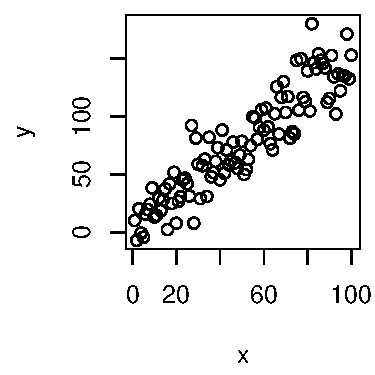
\includegraphics[bb=0in 0in 2.5in 2.5in, height=2.5in, width=2.5in]{Figure1.pdf}
    \label{fig:FigureAppendix}
\end{figure}

\section{Appendix Title B}
\label{app:AppendixLableB}

The detailed results are shown in Table~\ref{tab:DeckedTable}. 

\begin{table}
  \begin{threeparttable}
    \caption{A More Complex Decked Table}
    \label{tab:DeckedTable}
    \begin{tabular}{@{}lrrr@{}}         \toprule
    Distribution type  & \multicolumn{2}{l}{Percentage of} & Total number   \\
                       & \multicolumn{2}{l}{targets with}  & of trials per  \\
                       & \multicolumn{2}{l}{segment in}    & participant    \\ \cmidrule(r){2-3}
                                    &  Onset  &  Coda            &          \\ \midrule
    Categorical -- onset\tabfnm{a}  &    100  &     0            &  196     \\
    Probabilistic                   &     80  &    20\tabfnm{*}  &  200     \\
    Categorical -- coda\tabfnm{b}   &      0  &   100\tabfnm{*}  &  196     \\ \midrule
    \end{tabular}
    \begin{tablenotes}[para,flushleft]
        {\small
            \textit{Note.} All data are approximate.

            \tabfnt{a}Categorical may be onset.
            \tabfnt{b}Categorical may also be coda.

            \tabfnt{*}\textit{p} < .05.
            \tabfnt{**}\textit{p} < .01.
         }
    \end{tablenotes}
  \end{threeparttable}
\end{table}


\end{document}

%% 
%% Copyright (C) 2019 by Daniel A. Weiss <daniel.weiss.led at gmail.com>
%% 
%% This work may be distributed and/or modified under the
%% conditions of the LaTeX Project Public License (LPPL), either
%% version 1.3c of this license or (at your option) any later
%% version.  The latest version of this license is in the file:
%% 
%% http://www.latex-project.org/lppl.txt
%% 
%% Users may freely modify these files without permission, as long as the
%% copyright line and this statement are maintained intact.
%% 
%% This work is not endorsed by, affiliated with, or probably even known
%% by, the American Psychological Association.
%% 
%% This work is "maintained" (as per LPPL maintenance status) by
%% Daniel A. Weiss.
%% 
%% This work consists of the file  apa7.dtx
%% and the derived files           apa7.ins,
%%                                 apa7.cls,
%%                                 apa7.pdf,
%%                                 README,
%%                                 APA7american.txt,
%%                                 APA7british.txt,
%%                                 APA7dutch.txt,
%%                                 APA7english.txt,
%%                                 APA7german.txt,
%%                                 APA7ngerman.txt,
%%                                 APA7greek.txt,
%%                                 APA7czech.txt,
%%                                 APA7turkish.txt,
%%                                 APA7endfloat.cfg,
%%                                 Figure1.pdf,
%%                                 shortsample.tex,
%%                                 longsample.tex, and
%%                                 bibliography.bib.
%% 
%%
%% End of file `./samples/longsample.tex'.
